\documentclass[a4paper,titlepage]{article}

\usepackage{fullpage}

\usepackage[T1]{fontenc}
\usepackage[utf8]{inputenc}
\usepackage[spanish]{babel}
\usepackage{pdfpages}

\begin{document}

\title{Algorítmos y Estructuras de Datos II\\
Trabajo Práctico 2 (Diseño)\\
Grupo 6}

\author{
  Bayardo, Julián\\
  julian@bayardo.com.ar\\
  \texttt{850/13}
  \and
  Cuneo, Christian\\
  chriscuneo93@gmail.com\\
  \texttt{755/13}
  \and
  Gambaccini, Ezequiel\\
  ezequiel.gambaccini@gmail.com\\
  \texttt{715/13}
  \and
  Lebrero Rial, Ignacio Manuel\\
  ignaciolebrero@gmail.com\\
  \texttt{751/13}
}

\date{28 de Octubre del 2014}

\maketitle

%%%%%%%%%%%%%%%%%%%%%%%%%%%%%%%%%%%%%%%%%%%%%%%%%%%%%%%%%%%%%%%%%%%%%%%%%%%%%%%
%%%%						Aca empieza el documento
%%%%%%%%%%%%%%%%%%%%%%%%%%%%%%%%%%%%%%%%%%%%%%%%%%%%%%%%%%%%%%%%%%%%%%%%%%%%%%%
\section{Aclaraciones}
Como en ciudad se debe devolver una copia de mapa, hubo que implementar Copiar
en DiccString. Para copiar DiccString, hay que exigir que el parametro ($\alpha$)
de entrada tenga operacion copiar. Esto fue implementado en Restriccion, DiccString
y Cola de prioridad. No pudimos implementarlo en robot ya que para Copiar un robot,
se debe tener un iterador a la cola nueva, pero esto requeriria que Cola de prioridad
sepa mas cosas de su parametro de las que deberia.
La otra opcion era realizar una copia de robot con un iterador que no apunte a nada,
pero que no tendria sentido para robot.
%%%%%%%%%%%%%%%%%%%%%%%%%%%%%%%%%%%%%%%%%%%%%%%%%%%%%%%%%%%%%%%%%%%%%%%%%%%%%%%
%%%%                Iterador de Vector a Puntero
%%%%%%%%%%%%%%%%%%%%%%%%%%%%%%%%%%%%%%%%%%%%%%%%%%%%%%%%%%%%%%%%%%%%%%%%%%%%%%%
\section{Módulo Iterador de Vector a Puntero ($\alpha$)}

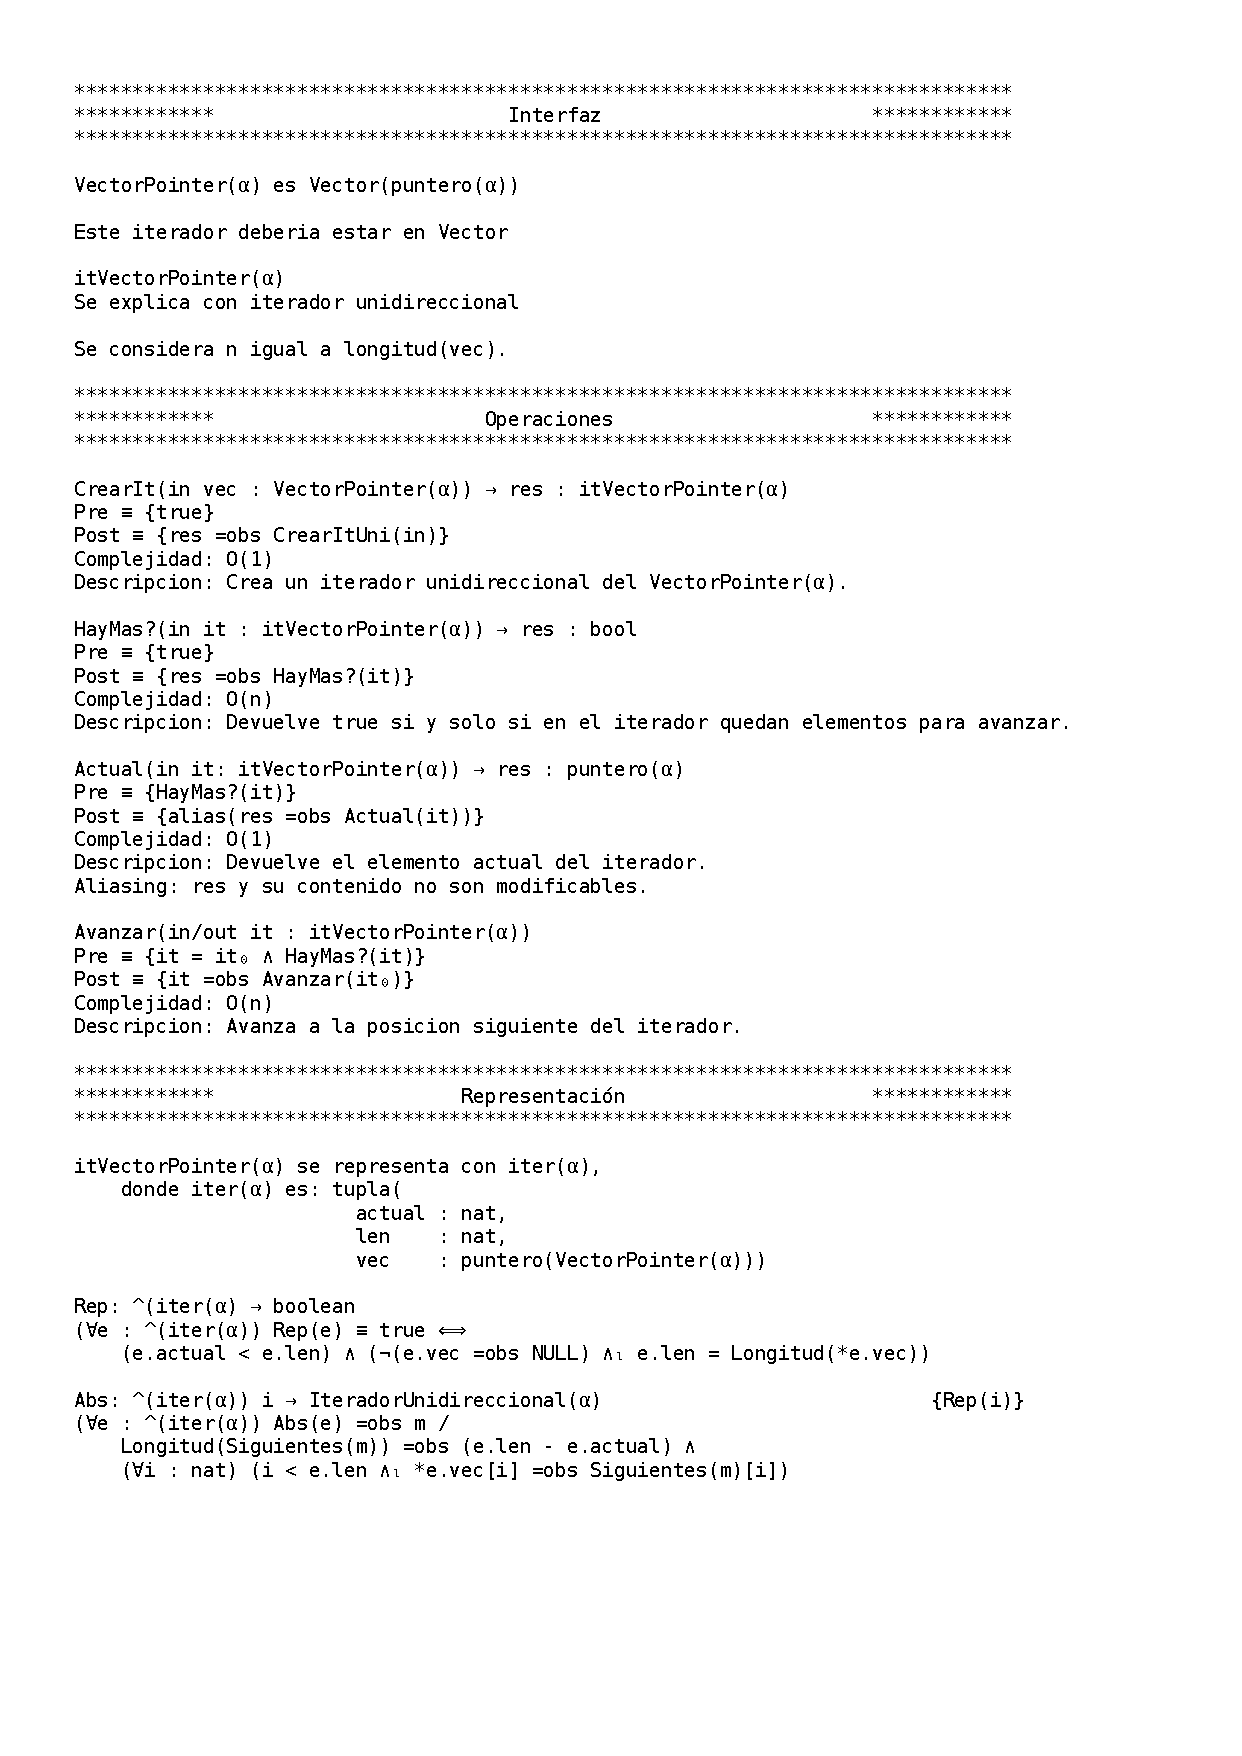
\includepdf[pages={1-}]{IteradorVectorPointer.pdf}

%%%%%%%%%%%%%%%%%%%%%%%%%%%%%%%%%%%%%%%%%%%%%%%%%%%%%%%%%%%%%%%%%%%%%%%%%%%%%%%
%%%%                Conjunto
%%%%%%%%%%%%%%%%%%%%%%%%%%%%%%%%%%%%%%%%%%%%%%%%%%%%%%%%%%%%%%%%%%%%%%%%%%%%%%%
\section{Módulo Conjunto Rápido de Strings}

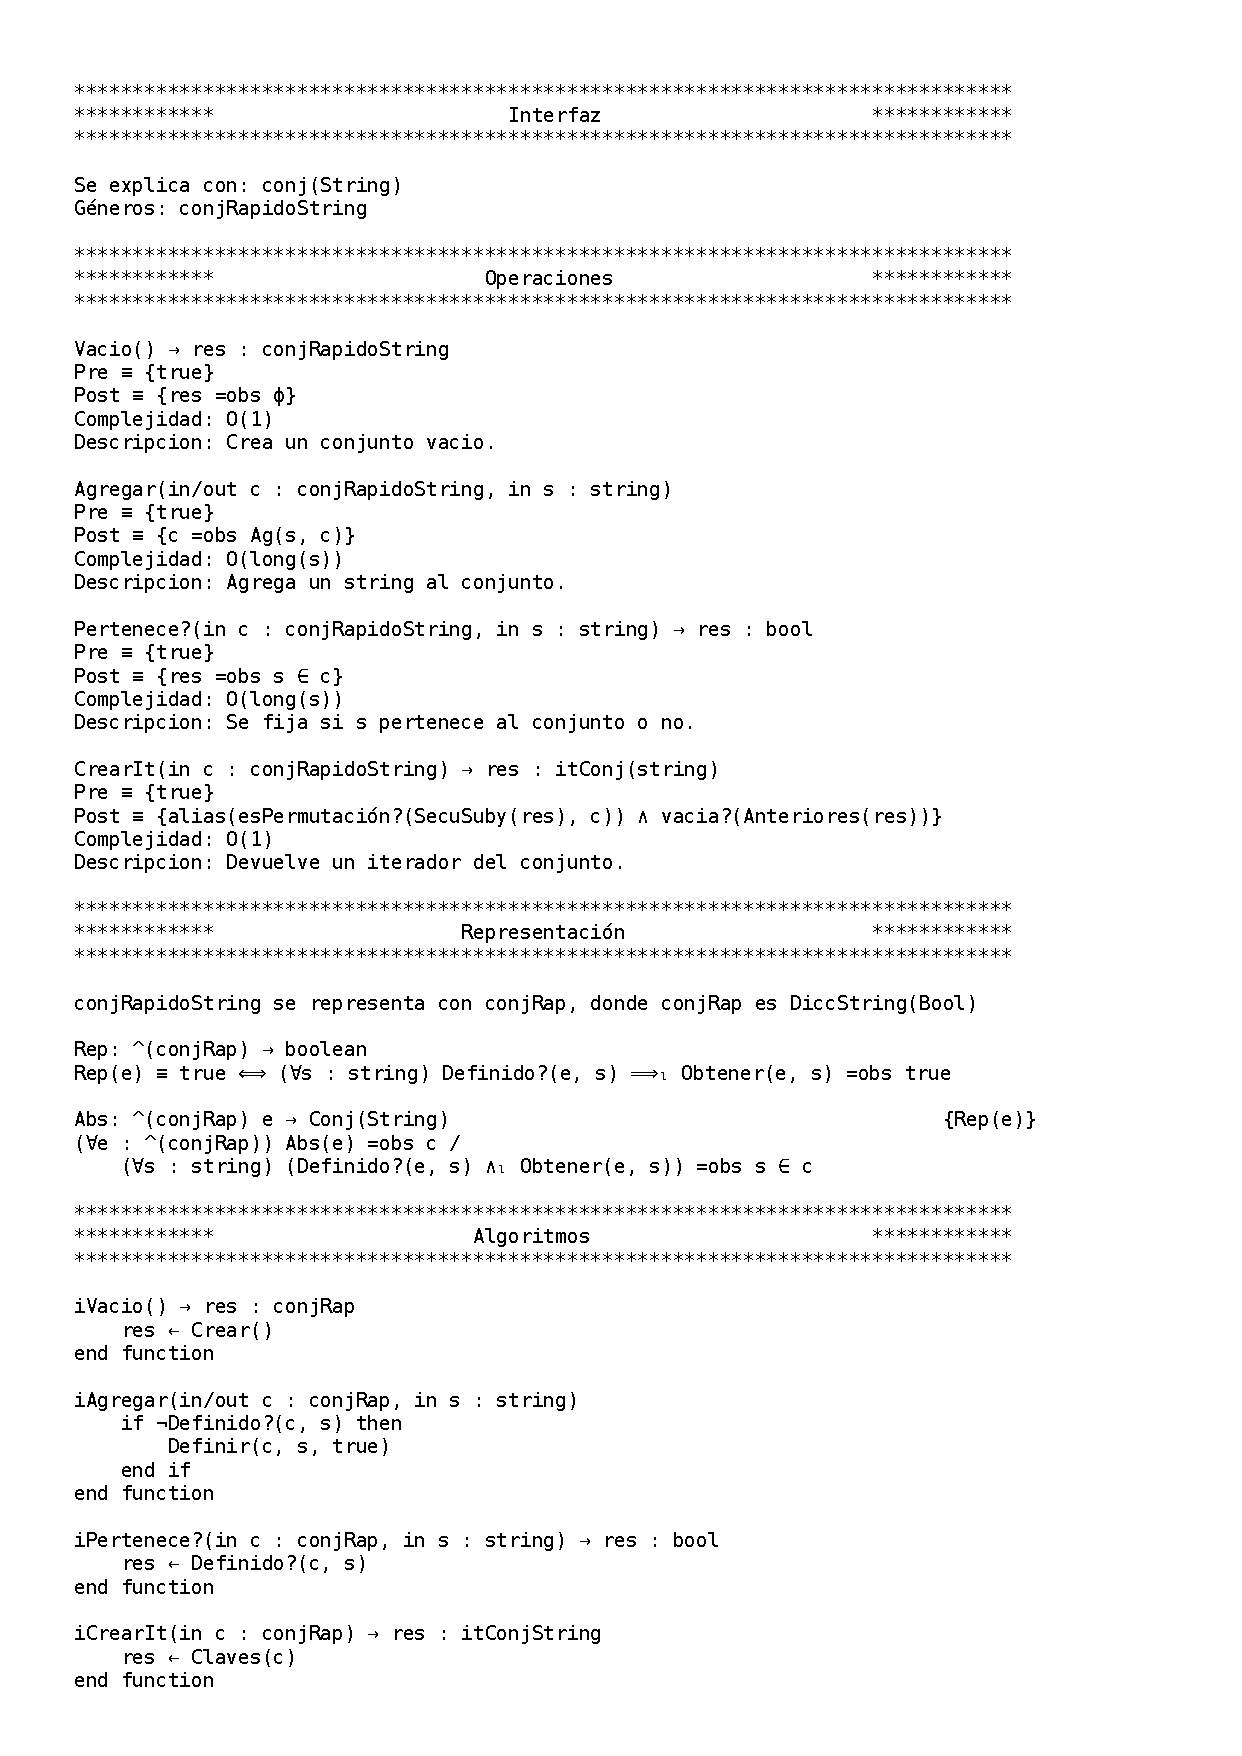
\includepdf[pages={1-}]{ConjuntoRapidoStrings.pdf}

%%%%%%%%%%%%%%%%%%%%%%%%%%%%%%%%%%%%%%%%%%%%%%%%%%%%%%%%%%%%%%%%%%%%%%%%%%%%%%%
%%%%								Trie
%%%%%%%%%%%%%%%%%%%%%%%%%%%%%%%%%%%%%%%%%%%%%%%%%%%%%%%%%%%%%%%%%%%%%%%%%%%%%%%
\section{Módulo Diccionario de Strings ($\alpha$)}

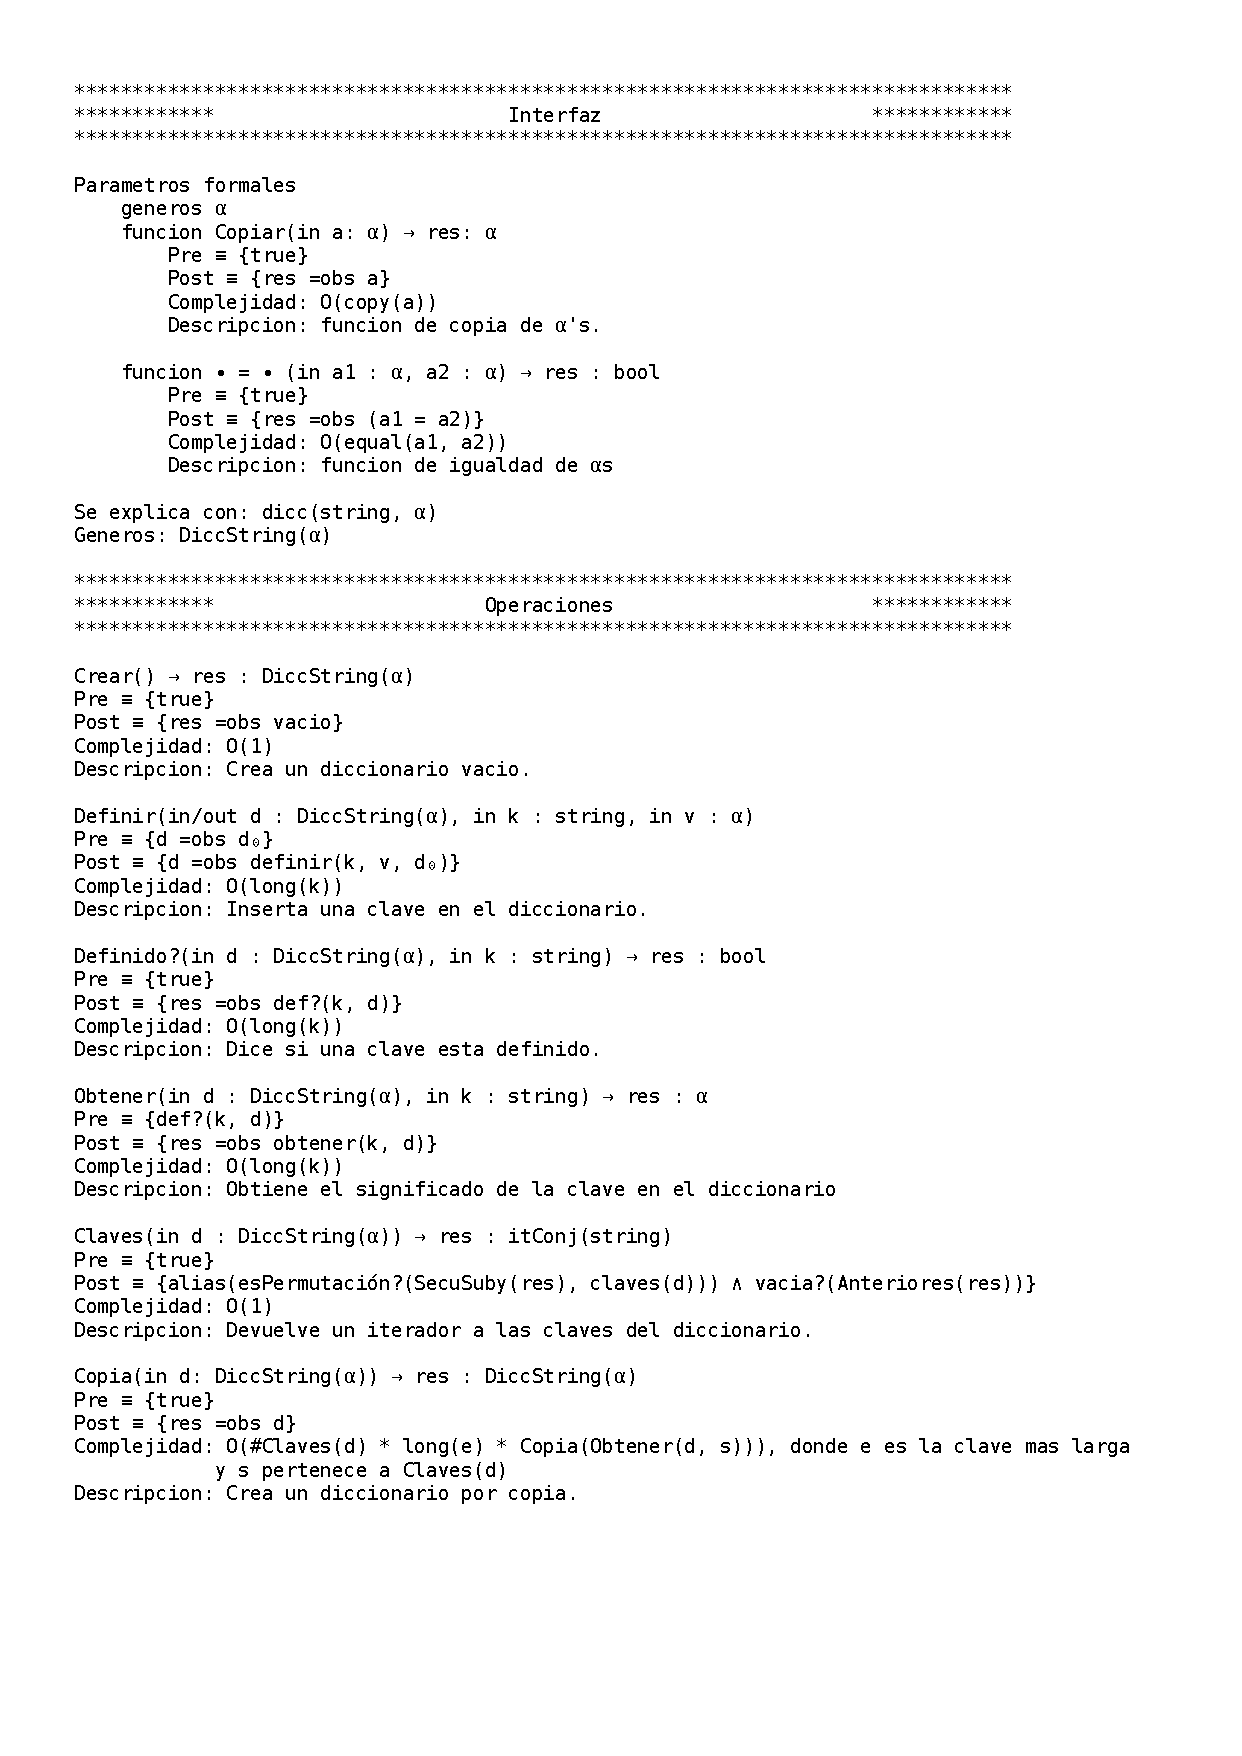
\includepdf[pages={1-}]{Diccionario.pdf}

%%%%%%%%%%%%%%%%%%%%%%%%%%%%%%%%%%%%%%%%%%%%%%%%%%%%%%%%%%%%%%%%%%%%%%%%%%%%%%%
%%%%							Cola de Prioridad
%%%%%%%%%%%%%%%%%%%%%%%%%%%%%%%%%%%%%%%%%%%%%%%%%%%%%%%%%%%%%%%%%%%%%%%%%%%%%%%
\section{Módulo Cola de Prioridad($\alpha$)}

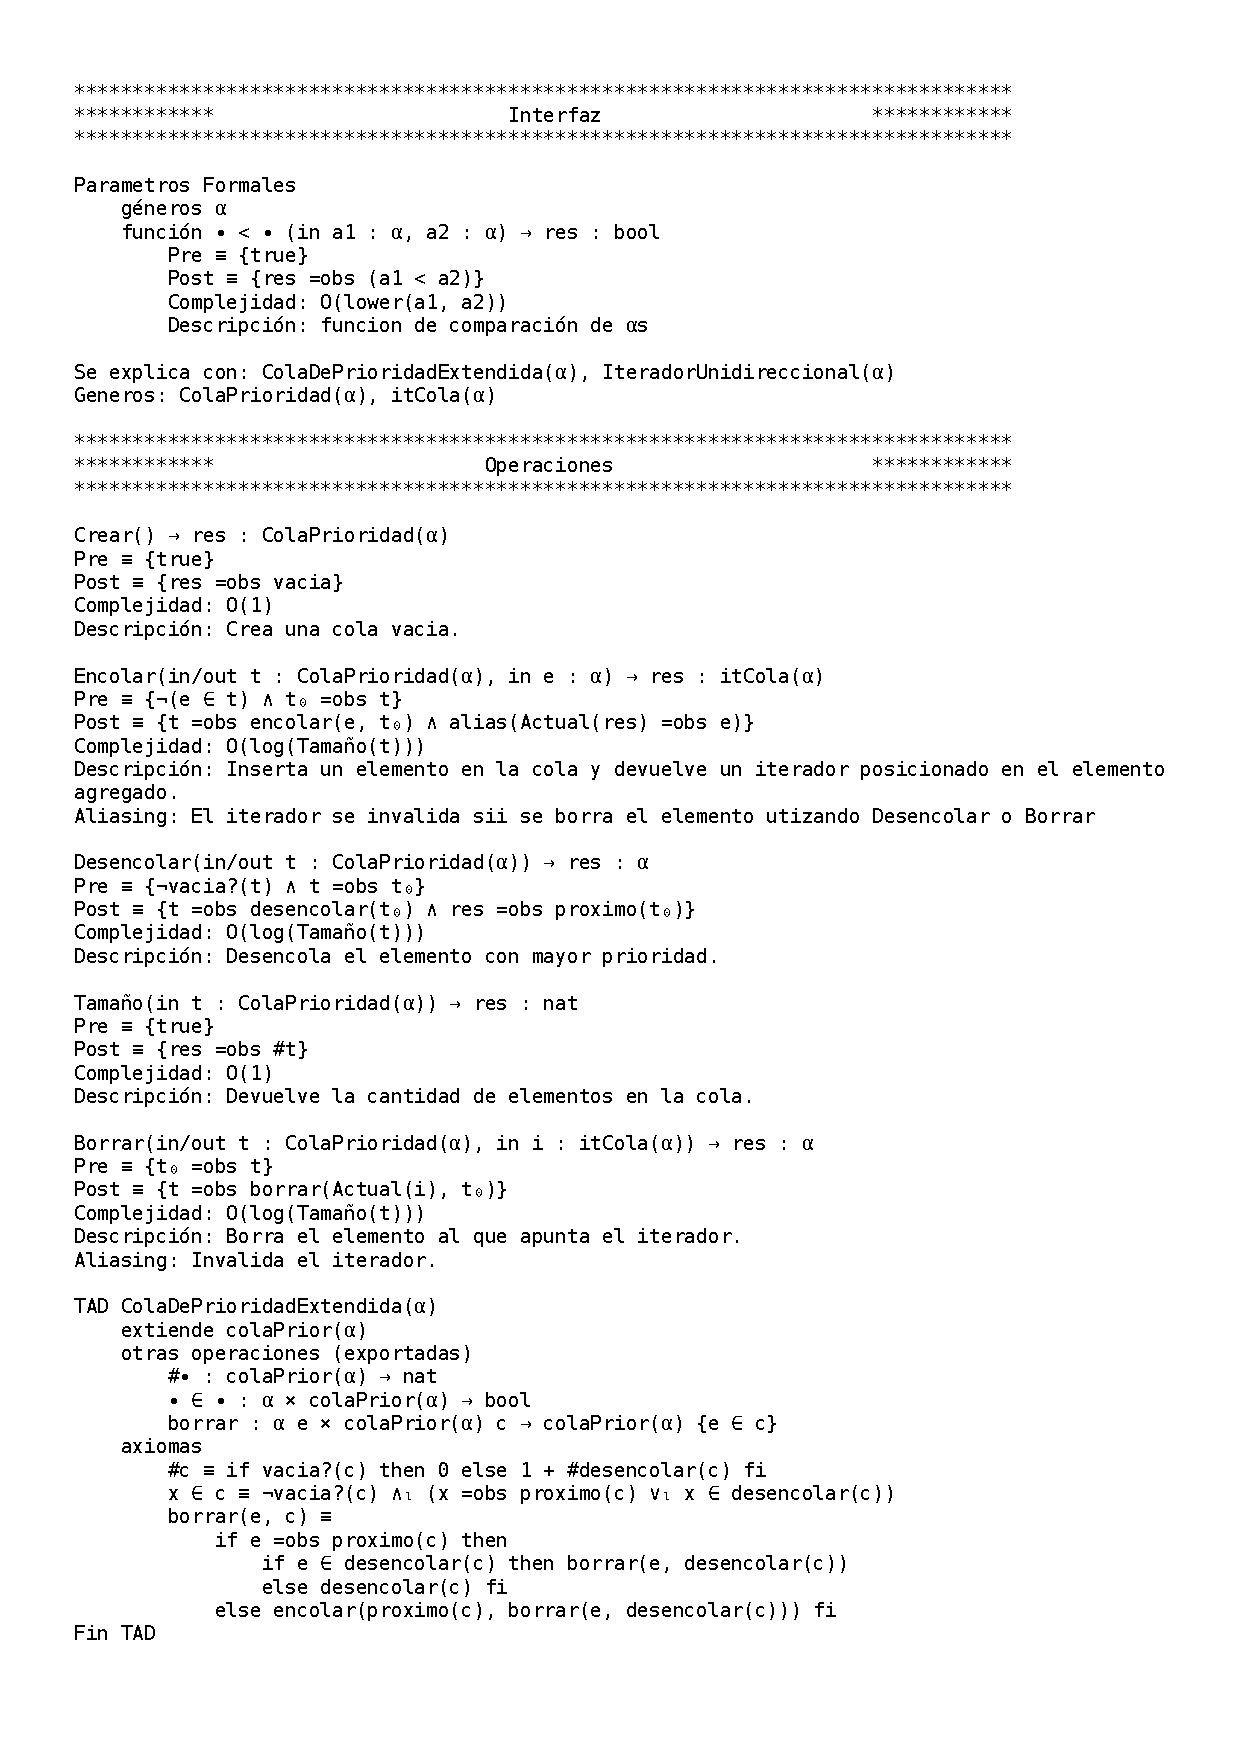
\includepdf[pages={1-}]{ColaDePrioridad.pdf}

%%%%%%%%%%%%%%%%%%%%%%%%%%%%%%%%%%%%%%%%%%%%%%%%%%%%%%%%%%%%%%%%%%%%%%%%%%%%%%%
%%%%							Restricción
%%%%%%%%%%%%%%%%%%%%%%%%%%%%%%%%%%%%%%%%%%%%%%%%%%%%%%%%%%%%%%%%%%%%%%%%%%%%%%%
\section{Módulo Restricción}

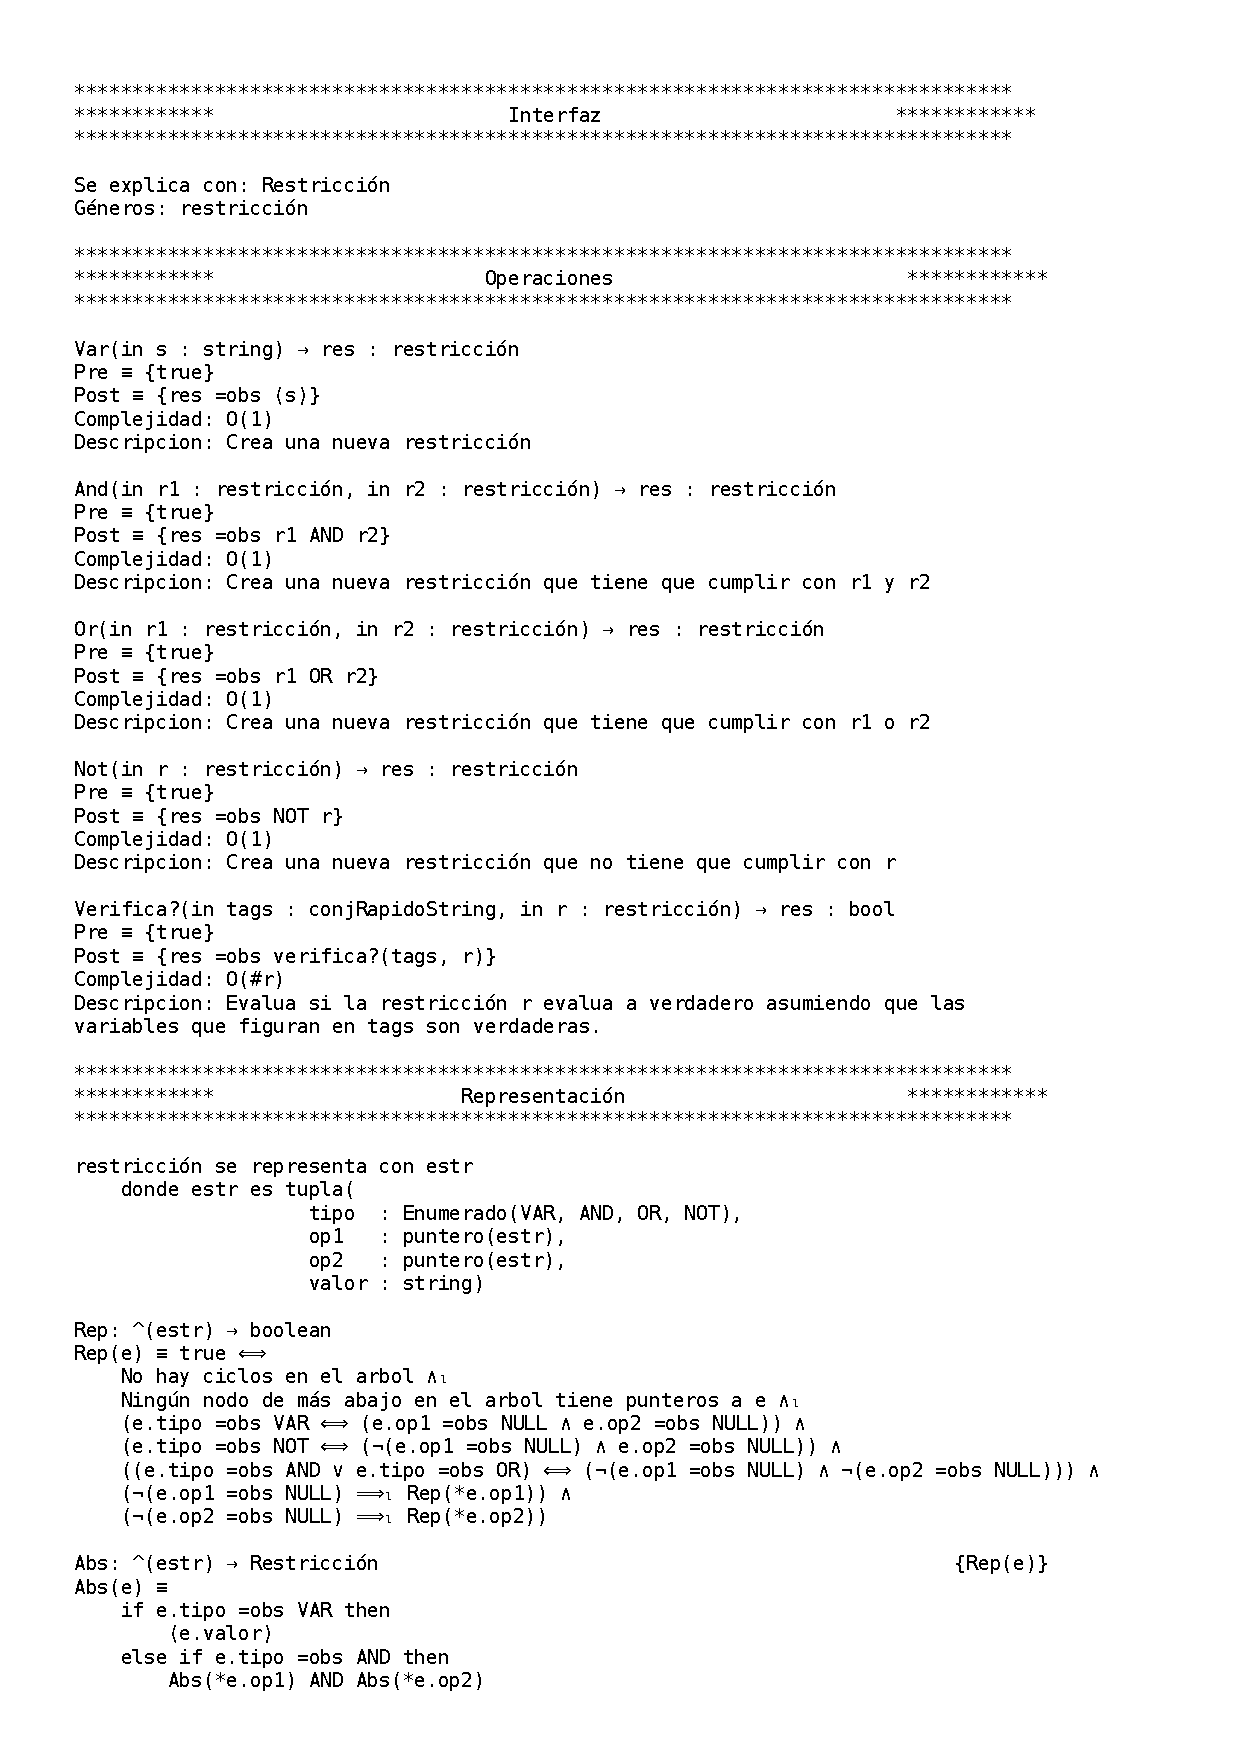
\includepdf[pages={1-}]{Restriccion.pdf}

%%%%%%%%%%%%%%%%%%%%%%%%%%%%%%%%%%%%%%%%%%%%%%%%%%%%%%%%%%%%%%%%%%%%%%%%%%%%%%%
%%%%								Mapa
%%%%%%%%%%%%%%%%%%%%%%%%%%%%%%%%%%%%%%%%%%%%%%%%%%%%%%%%%%%%%%%%%%%%%%%%%%%%%%%
\section{Módulo Mapa}

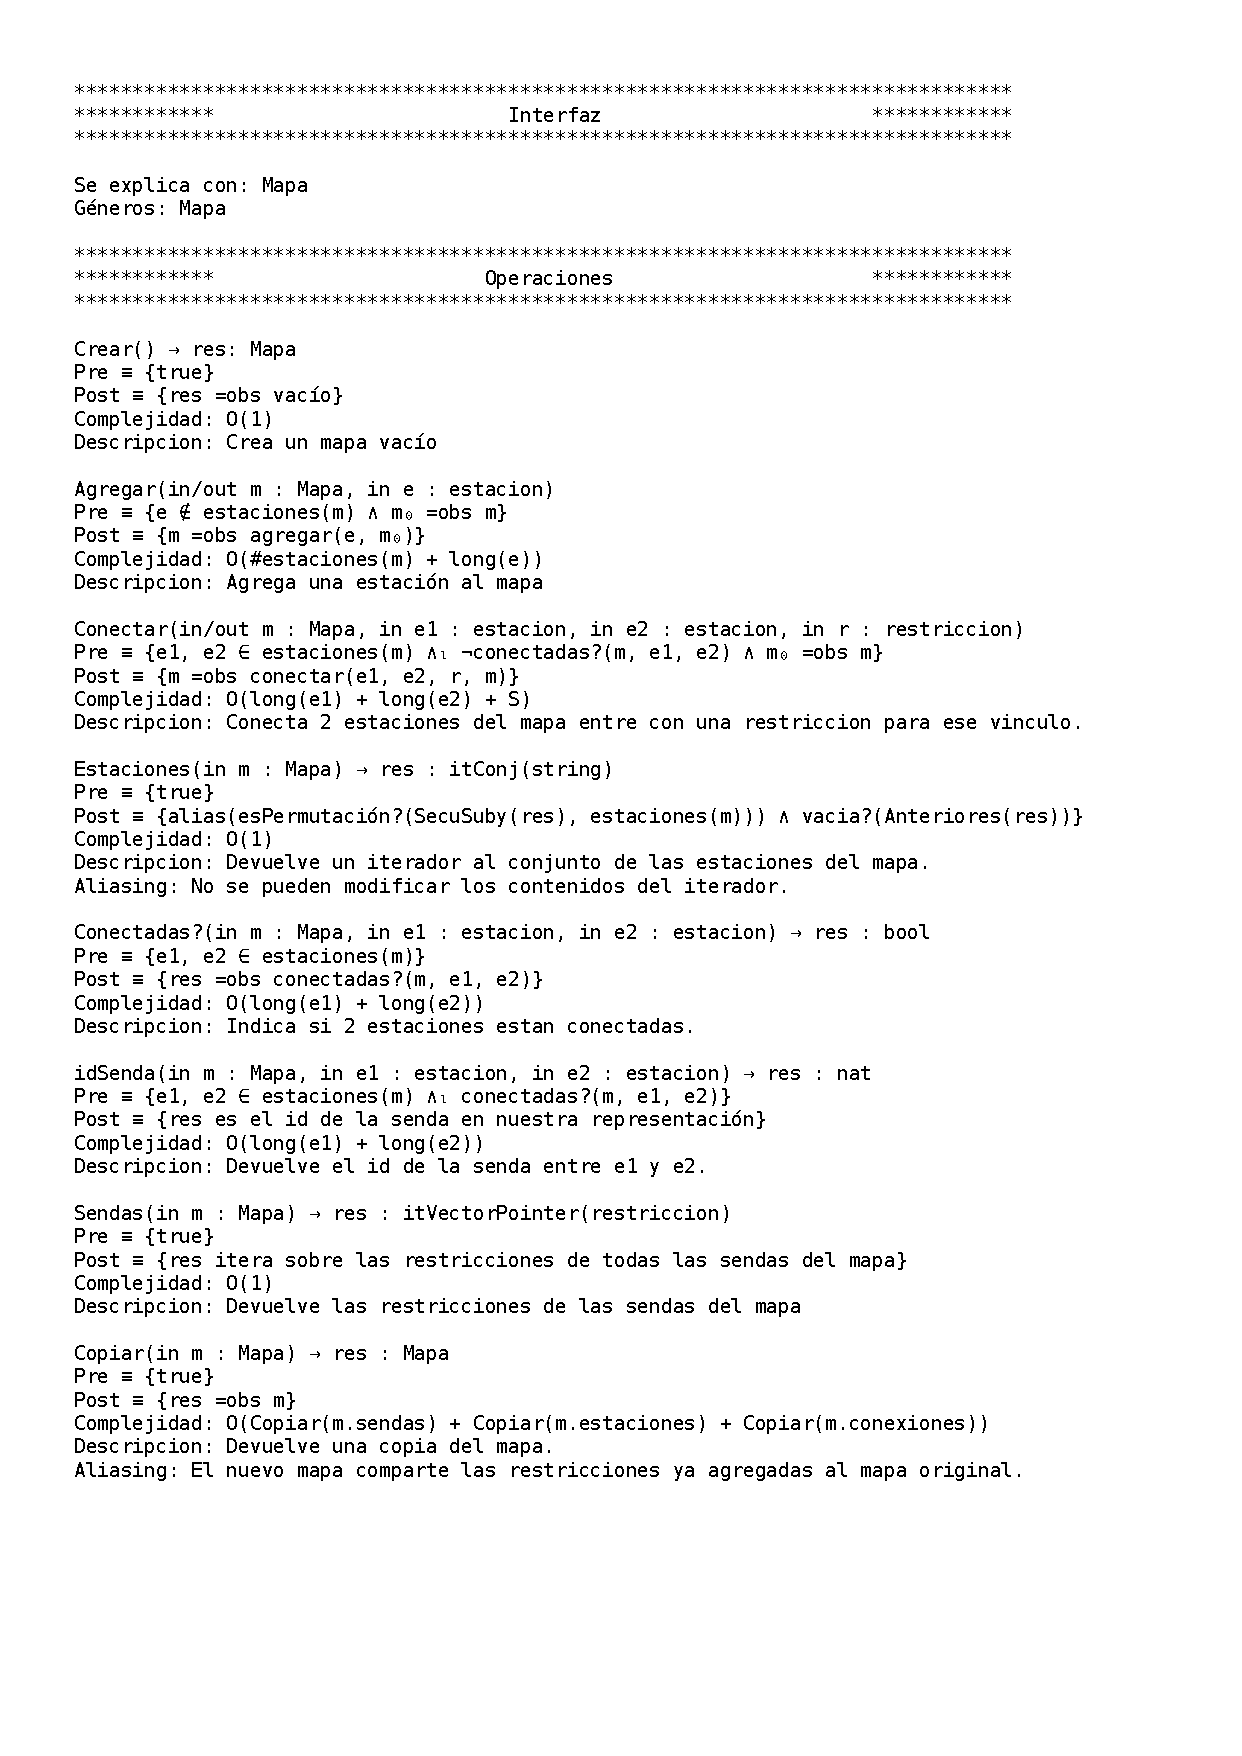
\includepdf[pages={1-}]{Mapa.pdf}

%%%%%%%%%%%%%%%%%%%%%%%%%%%%%%%%%%%%%%%%%%%%%%%%%%%%%%%%%%%%%%%%%%%%%%%%%%%%%%%
%%%%								Ciudad
%%%%%%%%%%%%%%%%%%%%%%%%%%%%%%%%%%%%%%%%%%%%%%%%%%%%%%%%%%%%%%%%%%%%%%%%%%%%%%%
\section{Módulo Ciudad}

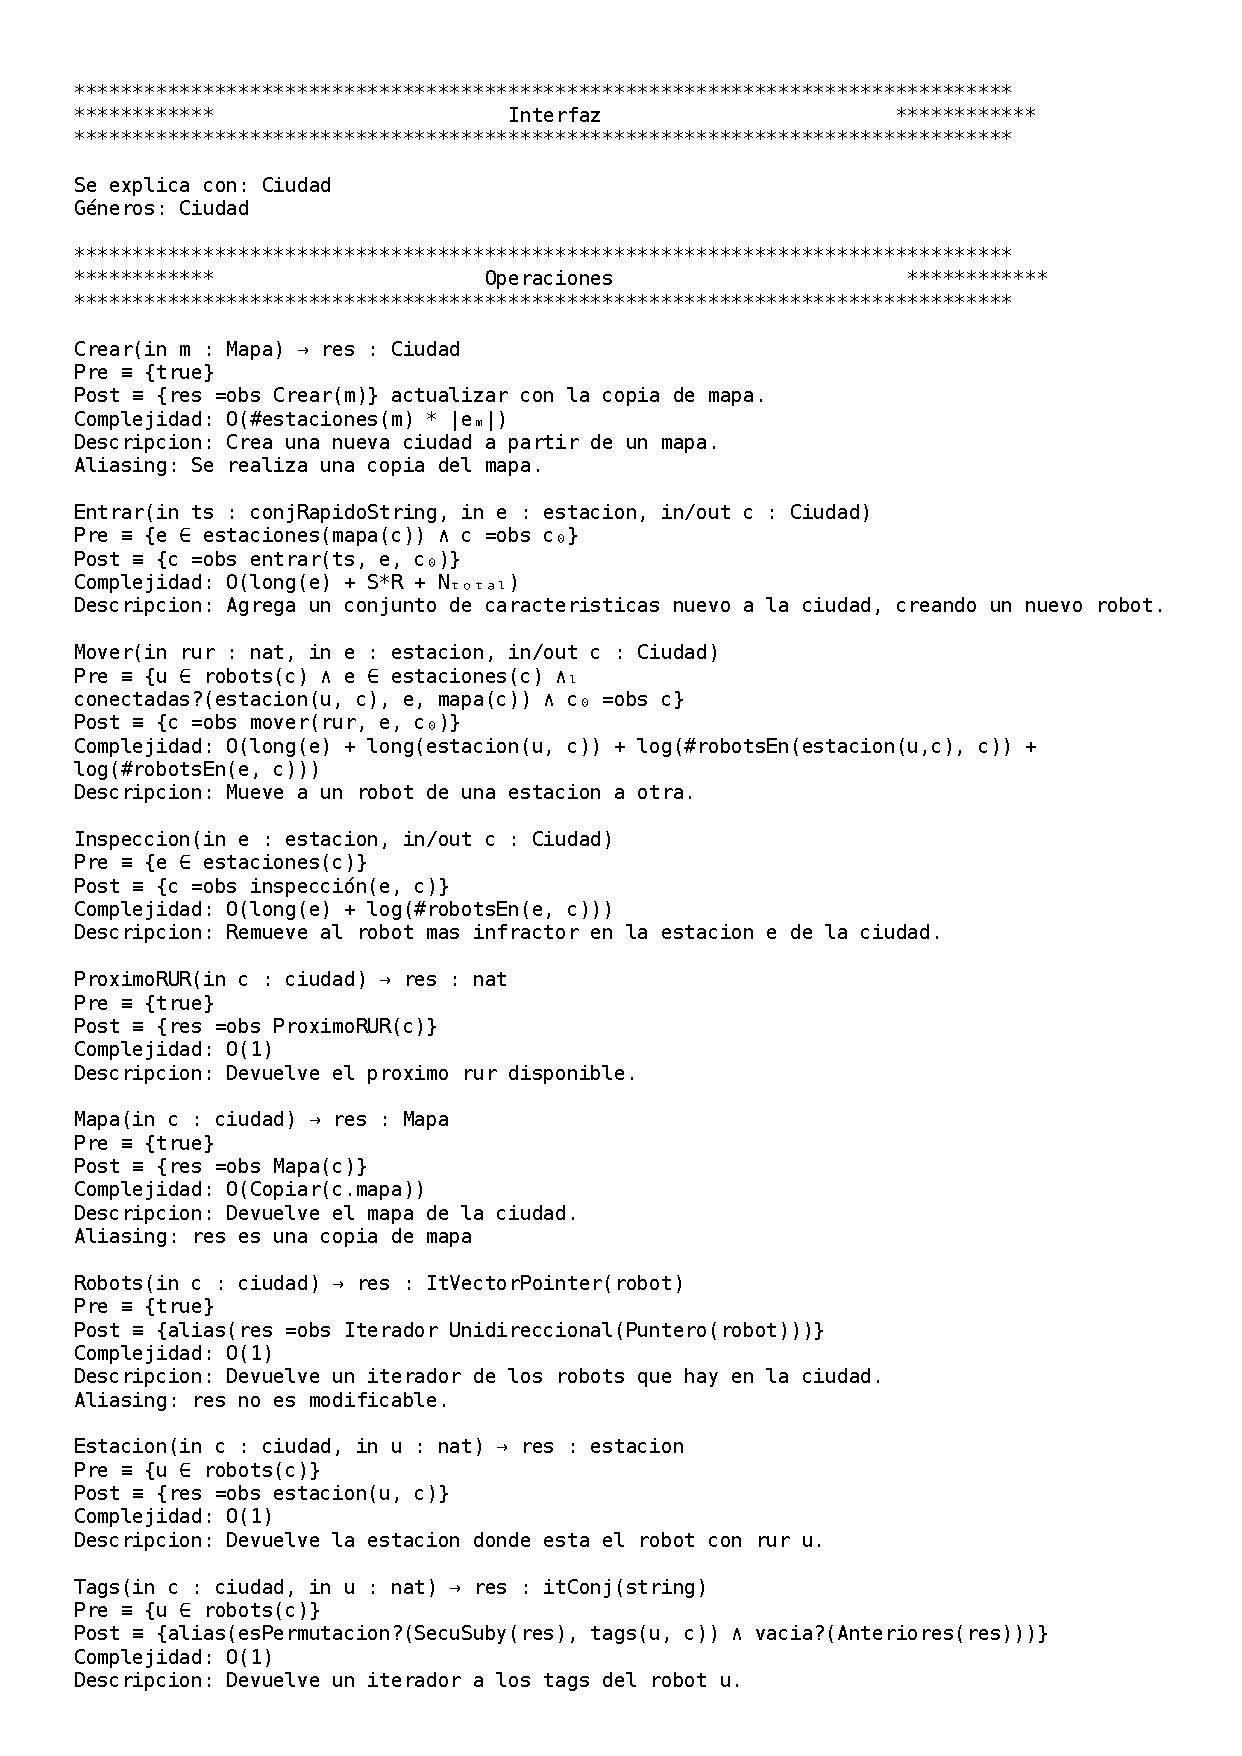
\includepdf[pages={1-}]{Ciudad.pdf}

\end{document}
